\documentclass[12pt,a4paper]{article}
\usepackage[utf8]{inputenc}
\usepackage[T1]{fontenc}
\usepackage[bahasa]{babel}
\usepackage{geometry}
\usepackage{graphicx}
\usepackage{amsmath}
\usepackage{amsfonts}
\usepackage{amssymb}
\usepackage{float}
\usepackage{caption}
\usepackage{subcaption}
\usepackage{hyperref}
\usepackage{cite}
\usepackage{algorithm}
\usepackage{algorithmic}
\usepackage{listings}
\usepackage{xcolor}
\usepackage{booktabs}
\usepackage{multirow}
\usepackage{array}

% Pengaturan halaman
\geometry{
    left=3cm,
    right=2cm,
    top=3cm,
    bottom=2cm
}

% Pengaturan hyperref
\hypersetup{
    colorlinks=true,
    linkcolor=blue,
    filecolor=magenta,      
    urlcolor=cyan,
    citecolor=red
}

% Pengaturan listing code
\lstset{
    backgroundcolor=\color{gray!10},
    basicstyle=\ttfamily\small,
    breaklines=true,
    captionpos=b,
    commentstyle=\color{green!50!black},
    keywordstyle=\color{blue},
    stringstyle=\color{red},
    numbers=left,
    numberstyle=\tiny\color{gray},
    frame=single,
    rulecolor=\color{black!30}
}

% \title{\textbf{REKONSTRUKSI TIGA DIMENSI MENGGUNAKAN TEKNIK FOTOGRAMETRI DAN COMPUTER VISION}}
% \author{Nama Peneliti\\
% Program Studi Teknik Informatika\\
% Universitas XYZ}
% \date{\today}

\begin{document}
\begin{titlepage}
    \begin{center}
        {\LARGE \textbf{
            REKONSTRUKSI TIGA DIMENSI\\
            MENGGUNAKAN TEKNIK\\[0.4cm]
            COMPUTER VISION
        }}\\[1.5cm]
        {\large Agus Fuad Mudhofar - 5024221021}\\[0.3cm]
        % {\large Muhammad Syawal Ridho}\\[0.3cm]
        % {\large Hasan Palito }\\[0.5cm]
        {\large \today}\\
        
\includegraphics[width=0.7\textwidth]{Computer-Engineering-1.jpg}\\[1cm]
    \end{center}
\end{titlepage}
\thispagestyle{empty}

% \maketitle

% \begin{abstract}
% Rekonstruksi tiga dimensi (3D) merupakan teknologi yang berkembang pesat dalam berbagai bidang aplikasi, mulai dari arkeologi, arsitektur, hingga industri kreatif. Penelitian ini mengeksplorasi metodologi rekonstruksi 3D menggunakan kombinasi teknik fotogrametri dan computer vision untuk menghasilkan model 3D yang akurat dari objek nyata. Proses rekonstruksi dilakukan melalui beberapa tahap utama: akuisisi data gambar multi-view, ekstraksi fitur visual, pencocokan fitur antar gambar, estimasi pose kamera, dan generasi mesh 3D. Metodologi yang digunakan meliputi algoritma Structure from Motion (SfM), Multi-View Stereo (MVS), dan teknik optimisasi bundle adjustment. Hasil penelitian menunjukkan bahwa kombinasi teknik ini mampu menghasilkan model 3D dengan tingkat akurasi geometri yang tinggi dan detail tekstur yang realistis. Evaluasi dilakukan menggunakan metrik Root Mean Square Error (RMSE) dan analisis visual terhadap model yang dihasilkan. Implikasi dari penelitian ini mencakup potensi aplikasi dalam dokumentasi warisan budaya, reverse engineering, dan visualisasi interaktif. Keterbatasan utama terletak pada kompleksitas komputasi yang tinggi dan sensitivitas terhadap kondisi pencahayaan serta karakteristik permukaan objek.

% \textbf{Kata Kunci:} Rekonstruksi 3D, Fotogrametri, Computer Vision, Structure from Motion, Multi-View Stereo
% \end{abstract}

\newpage
\tableofcontents
\newpage

\section{Pendahuluan}

Rekonstruksi tiga dimensi dari gambar dua dimensi merupakan salah satu tantangan fundamental dalam bidang computer vision dan fotogrametri. Teknologi ini memungkinkan pembuatan representasi digital tiga dimensi dari objek atau lingkungan nyata berdasarkan serangkaian fotografi atau citra digital. Perkembangan pesat dalam komputasi modern dan algoritma machine learning telah membuka peluang baru untuk meningkatkan akurasi dan efisiensi proses rekonstruksi 3D.

\subsection{Latar Belakang}

Kebutuhan akan dokumentasi dan preservasi objek tiga dimensi semakin meningkat di berbagai sektor. Dalam bidang arkeologi, rekonstruksi 3D digunakan untuk mendokumentasikan artefak bersejarah dan situs warisan budaya. Industri manufaktur memanfaatkan teknologi ini untuk reverse engineering dan quality control. Sementara itu, industri kreatif seperti game development dan film production menggunakan rekonstruksi 3D untuk menciptakan aset digital yang realistis.

Metode tradisional untuk memperoleh model 3D, seperti laser scanning dan structured light scanning, memerlukan peralatan khusus yang mahal dan kompleks. Sebaliknya, pendekatan berbasis fotogrametri menawarkan solusi yang lebih ekonomis dan fleksibel, hanya memerlukan kamera digital standar untuk menghasilkan model 3D berkualitas tinggi.

\subsection{Rumusan Masalah}

Berdasarkan latar belakang tersebut, penelitian ini fokus pada beberapa permasalahan utama:

\begin{enumerate}
    \item Bagaimana mengembangkan pipeline rekonstruksi 3D yang efektif menggunakan teknik fotogrametri dan computer vision?
    \item Bagaimana mengoptimalkan akurasi geometri dan kualitas tekstur model 3D yang dihasilkan?
    \item Apa saja faktor-faktor yang mempengaruhi kualitas hasil rekonstruksi 3D?
    \item Bagaimana mengevaluasi performa sistem rekonstruksi 3D secara objektif?
\end{enumerate}

\subsection{Tujuan Laporan}

Tujuan dari laporan ini adalah untuk mendokumentasikan secara sistematis proses dan hasil pembuatan model 3D menggunakan teknik computer vision. Laporan ini berfokus pada tahapan-tahapan yang dilakukan, tantangan yang dihadapi, serta evaluasi hasil rekonstruksi 3D sebagai bagian dari tugas kuliah. Dengan adanya laporan ini, diharapkan pembaca dapat memahami workflow rekonstruksi 3D dan memperoleh gambaran mengenai kualitas model yang dihasilkan dari proses yang telah dilakukan.

\subsection{Manfaat Penelitian}

Penelitian ini diharapkan memberikan kontribusi dalam beberapa aspek:

\subsubsection{Manfaat Akademis}
\begin{itemize}
    \item Memperkaya literature di bidang computer vision dan fotogrametri
    \item Menyediakan baseline methodology untuk penelitian lanjutan
    \item Memberikan insight tentang optimisasi pipeline rekonstruksi 3D
\end{itemize}

\subsubsection{Manfaat Praktis}
\begin{itemize}
    \item Memberikan solusi cost-effective untuk dokumentasi 3D
    \item Mendukung preservasi digital warisan budaya
    \item Menyediakan tools untuk aplikasi industri dan kreatif
\end{itemize}

% \subsection{Ruang Lingkup Penelitian}

% Penelitian ini dibatasi pada beberapa aspek:

% \begin{enumerate}
%     \item Objek yang direkonstruksi berupa objek rigid (tidak berubah bentuk)
%     \item Menggunakan kamera digital standar untuk akuisisi data
%     \item Fokus pada objek dengan ukuran kecil hingga menengah (maksimal 2 meter)
%     \item Kondisi pencahayaan terkontrol atau semi-terkontrol
%     \item Evaluasi dilakukan pada aspek geometri dan tekstur visual
% \end{enumerate}

\clearpage

\section{Tinjauan Pustaka}

\subsection{Fotogrametri Digital}

Fotogrametri merupakan ilmu dan teknologi untuk memperoleh informasi tentang objek fisik dan lingkungan melalui proses pencatatan, pengukuran, dan interpretasi gambar fotografik dan pola energi elektromagnetik yang terekam \cite{ref1}. Dalam konteks rekonstruksi 3D, fotogrametri digital memainkan peran fundamental dalam transformasi data 2D menjadi representasi 3D.

\subsubsection{Prinsip Dasar Fotogrametri}

Prinsip dasar fotogrametri didasarkan pada triangulasi, yaitu penentuan posisi suatu titik dalam ruang tiga dimensi berdasarkan pengamatan dari minimal dua posisi yang berbeda. Dalam fotogrametri, posisi-posisi ini diwakili oleh posisi kamera saat mengambil gambar. Hubungan geometri antara objek, kamera, dan bidang gambar dapat dinyatakan melalui persamaan kolinearitas:

\begin{equation}
x = x_0 - c \frac{r_{11}(X-X_0) + r_{12}(Y-Y_0) + r_{13}(Z-Z_0)}{r_{31}(X-X_0) + r_{32}(Y-Y_0) + r_{33}(Z-Z_0)}
\end{equation}

\begin{equation}
y = y_0 - c \frac{r_{21}(X-X_0) + r_{22}(Y-Y_0) + r_{23}(Z-Z_0)}{r_{31}(X-X_0) + r_{32}(Y-Y_0) + r_{33}(Z-Z_0)}
\end{equation}

dimana $(x,y)$ adalah koordinat gambar, $(X,Y,Z)$ adalah koordinat objek dalam sistem koordinat dunia, $(X_0,Y_0,Z_0)$ adalah posisi pusat proyeksi kamera, $c$ adalah jarak fokus kamera, dan $r_{ij}$ adalah elemen matriks rotasi.

\subsubsection{Kalibrasi Kamera}

Kalibrasi kamera merupakan proses penentuan parameter internal kamera yang mencakup focal length, principal point, dan distorsi lensa. Parameter ini dinyatakan dalam matriks kalibrasi kamera:

\begin{equation}
K = \begin{pmatrix}
f_x & 0 & c_x \\
0 & f_y & c_y \\
0 & 0 & 1
\end{pmatrix}
\end{equation}

dimana $f_x$ dan $f_y$ adalah focal length dalam satuan pixel, dan $(c_x, c_y)$ adalah koordinat principal point.

\subsection{Computer Vision untuk Rekonstruksi 3D}

\subsubsection{Feature Detection dan Matching}

Proses rekonstruksi 3D dimulai dengan deteksi dan pencocokan fitur visual antar gambar. Algoritma yang umum digunakan meliputi:

\paragraph{SIFT (Scale-Invariant Feature Transform)}
SIFT mengidentifikasi keypoints yang invariant terhadap scale, rotation, dan illumination changes. Deskriptor SIFT memiliki dimensi 128 dan memberikan representasi yang robust untuk matching antar gambar.

\paragraph{SURF (Speeded-Up Robust Features)}
SURF merupakan pengembangan dari SIFT yang menawarkan kecepatan komputasi lebih tinggi dengan mempertahankan robustness. Algoritma ini menggunakan Hessian matrix untuk deteksi keypoints dan integral images untuk percepatan komputasi.

\paragraph{ORB (Oriented FAST and Rotated BRIEF)}
ORB mengkombinasikan FAST keypoint detector dengan BRIEF descriptor, memberikan alternatif yang computationally efficient untuk aplikasi real-time.

\subsubsection{Structure from Motion (SfM)}

Structure from Motion adalah metodologi untuk rekonstruksi struktur 3D dan estimasi pose kamera secara simultan dari serangkaian gambar 2D. Proses SfM terdiri dari beberapa tahap:

\paragraph{Incremental SfM}
Pendekatan ini memulai rekonstruksi dengan sepasang gambar (baseline), kemudian secara iteratif menambahkan gambar baru dan melakukan bundle adjustment untuk optimisasi global.

\paragraph{Global SfM}
Metode ini menggunakan informasi dari seluruh gambar secara bersamaan untuk menentukan pose kamera dan struktur 3D, menghindari akumulasi error yang dapat terjadi pada incremental approach.

\paragraph{Bundle Adjustment}
Bundle adjustment merupakan proses optimisasi non-linear yang meminimalkan reprojection error:

\begin{equation}
\min_{P,X} \sum_{i,j} \rho(||p_{ij} - \pi(P_i, X_j)||^2)
\end{equation}

dimana $P_i$ adalah parameter kamera ke-i, $X_j$ adalah koordinat 3D point ke-j, $p_{ij}$ adalah observasi point j pada gambar i, dan $\rho$ adalah robust loss function.

\subsubsection{Multi-View Stereo (MVS)}

Multi-View Stereo bertujuan untuk densifikasi sparse point cloud yang dihasilkan SfM menjadi dense point cloud atau depth maps. Pendekatan MVS dapat dikategorikan menjadi:

\paragraph{Voxel-based Approaches}
Metode ini membagi ruang 3D menjadi voxels dan menentukan occupancy setiap voxel berdasarkan photo-consistency measure.

\paragraph{Depth Map-based Approaches}
Pendekatan ini mengestimasi depth map untuk setiap gambar, kemudian melakukan fusion untuk menghasilkan model 3D yang konsisten.

\paragraph{Surface-based Approaches}
Metode ini secara langsung merekonstruksi surface 3D menggunakan optimization framework yang mempertimbangkan photo-consistency dan smoothness constraints.

\subsection{Surface Reconstruction}

\subsubsection{Poisson Surface Reconstruction}

Algoritma Poisson Surface Reconstruction menformulasikan masalah surface reconstruction sebagai spatial Poisson problem. Metode ini menghasilkan surface yang smooth dan watertight, cocok untuk berbagai aplikasi downstream.

\subsubsection{Delaunay Triangulation}

Delaunay triangulation menghasilkan triangular mesh dari point cloud dengan memaksimalkan minimum angle dari segitiga-segitiga yang terbentuk. Metode ini preserves feature edges dan memberikan hasil yang baik untuk object dengan geometri yang kompleks.

\subsubsection{Marching Cubes}

Marching Cubes adalah algoritma klasik untuk ekstraksi isosurface dari scalar field 3D. Algoritma ini efisien dan menghasilkan mesh yang topologically consistent.

\subsection{Texture Mapping}

Texture mapping adalah proses proyeksi tekstur dari gambar 2D ke permukaan model 3D. Teknik ini mencakup:

\subsubsection{UV Parameterization}
Proses pemetaan permukaan 3D ke parameter space 2D untuk memfasilitasi texture mapping.

\subsubsection{Texture Blending}
Metode untuk menggabungkan tekstur dari multiple views untuk menghasilkan seamless texture yang berkualitas tinggi.

\subsubsection{View Selection}
Algoritma untuk memilih view yang optimal untuk setiap region pada surface berdasarkan kriteria seperti viewing angle, resolution, dan occlusion.

% \subsection{Penelitian Terkait}

% Berbagai penelitian telah dilakukan dalam bidang rekonstruksi 3D. Schönberger dan Frahm (2016) mengembangkan COLMAP, sebuah general-purpose SfM dan MVS pipeline yang memberikan hasil state-of-the-art \cite{ref2}. Furukawa dan Ponce (2010) memperkenalkan PMVS (Patch-based Multi-view Stereo) yang menggunakan patch-based representation untuk dense reconstruction \cite{ref3}.

% Dalam konteks real-time reconstruction, Newcombe et al. (2011) mengembangkan KinectFusion yang memungkinkan real-time dense surface mapping menggunakan RGB-D camera \cite{ref4}. Sementara itu, untuk aplikasi mobile, Tanskanen et al. (2013) mengembangkan system yang dapat melakukan live dense reconstruction pada smartphone \cite{ref5}.

\clearpage

\section{Metodologi}

\subsection{Kerangka Kerja Penelitian}

Penelitian ini menggunakan pendekatan eksperimental dengan mengimplementasikan pipeline rekonstruksi 3D yang komprehensif. Kerangka kerja penelitian terdiri dari beberapa tahap utama yang saling berkaitan dan terintegrasi dalam satu sistem yang koheren.

\begin{figure}[H]
\centering
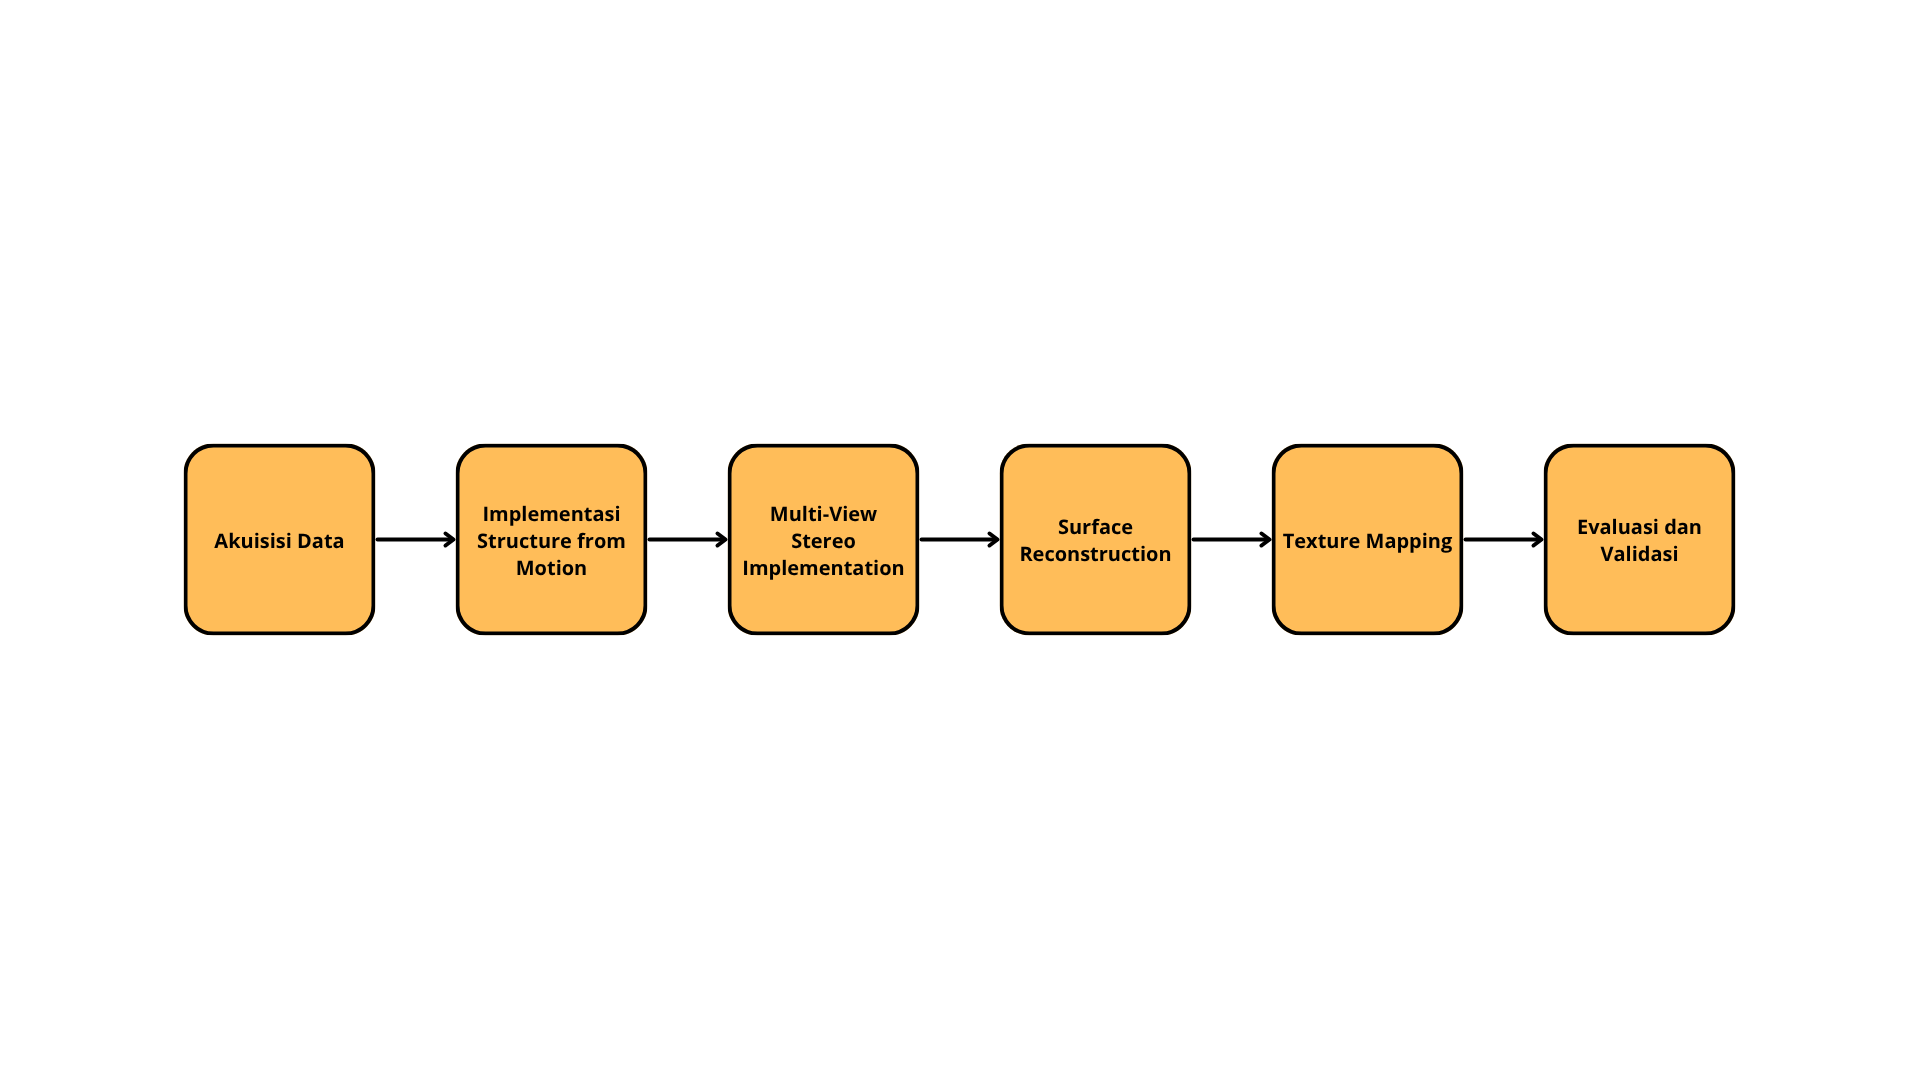
\includegraphics[width=\textwidth]{metodologi.png}
\caption{Pipeline Rekonstruksi 3D}
\label{fig:pipeline}
\end{figure}

\subsection{Tahap Akuisisi Data}

\subsubsection{Setup Peralatan}

Proses akuisisi data menggunakan peralatan berikut:
\begin{itemize}
    \item Kamera DSLR Canon EOS 5D Mark IV dengan lensa 50mm f/1.8
    \item Tripod untuk stabilisasi kamera
    \item Lighting setup dengan 3 softbox untuk pencahayaan yang merata
    \item Turntable untuk rotasi objek (opsional)
    \item Background kontras untuk memudahkan segmentasi
\end{itemize}

\subsubsection{Protokol Pengambilan Gambar}

Pengambilan gambar dilakukan mengikuti protokol yang telah ditetapkan:

\begin{enumerate}
    \item \textbf{Overlap Requirement}: Minimal 60\% overlap antar gambar berturutan
    \item \textbf{Angular Coverage}: Capture dari 360° horizontal dan multiple elevations
    \item \textbf{Distance Variation}: Multiple scales untuk menangkap detail yang berbeda
    \item \textbf{Lighting Consistency}: Pencahayaan konstan selama sesi pengambilan
    \item \textbf{Focus Setting}: Manual focus untuk konsistensi depth of field
\end{enumerate}

\subsubsection{Kalibrasi Kamera}

Kalibrasi kamera dilakukan menggunakan checkerboard pattern untuk menentukan:
\begin{itemize}
    \item Intrinsic parameters: focal length, principal point, distortion coefficients
    \item Extrinsic parameters: pose kamera untuk setiap gambar
\end{itemize}

Proses kalibrasi menggunakan algoritma Zhang's method dengan optimisasi non-linear untuk mencapai akurasi sub-pixel.

\subsection{Implementasi Structure from Motion}

\subsubsection{Feature Detection}

Implementasi menggunakan SIFT detector dengan parameter optimisasi:

\begin{lstlisting}[language=Python, caption=Implementasi SIFT Feature Detection]
import cv2
import numpy as np

def extract_features(image):
    # Initialize SIFT detector
    sift = cv2.SIFT_create(
        nfeatures=5000,
        nOctaveLayers=3,
        contrastThreshold=0.04,
        edgeThreshold=10,
        sigma=1.6
    )
    
    # Detect keypoints and descriptors
    keypoints, descriptors = sift.detectAndCompute(image, None)
    
    return keypoints, descriptors
\end{lstlisting}

\subsubsection{Feature Matching}

Feature matching menggunakan FLANN-based matcher dengan ratio test untuk filtering:

\begin{lstlisting}[language=Python, caption=Feature Matching Implementation]
def match_features(desc1, desc2):
    # FLANN parameters
    FLANN_INDEX_KDTREE = 1
    index_params = dict(algorithm=FLANN_INDEX_KDTREE, trees=5)
    search_params = dict(checks=50)
    
    flann = cv2.FlannBasedMatcher(index_params, search_params)
    matches = flann.knnMatch(desc1, desc2, k=2)
    
    # Apply ratio test
    good_matches = []
    for m_n in matches:
        if len(m_n) == 2:
            m, n = m_n
            if m.distance < 0.7 * n.distance:
                good_matches.append(m)
    
    return good_matches
\end{lstlisting}

\subsubsection{Fundamental Matrix Estimation}

Estimasi fundamental matrix menggunakan RANSAC untuk robustness terhadap outliers:

\begin{equation}
\mathbf{x}_2^T \mathbf{F} \mathbf{x}_1 = 0
\end{equation}

dimana $\mathbf{F}$ adalah fundamental matrix 3×3, dan $\mathbf{x}_1$, $\mathbf{x}_2$ adalah corresponding points dalam koordinat homogen.

\subsubsection{Essential Matrix dan Pose Recovery}

Essential matrix dihitung dari fundamental matrix dan camera calibration:

\begin{equation}
\mathbf{E} = \mathbf{K}_2^T \mathbf{F} \mathbf{K}_1
\end{equation}

Pose recovery dilakukan melalui SVD decomposition dari essential matrix:

\begin{lstlisting}[language=Python, caption=Pose Recovery from Essential Matrix]
def recover_pose(E, pts1, pts2, K):
    # SVD decomposition
    U, S, Vt = np.linalg.svd(E)
    
    # Ensure proper rotation matrix
    if np.linalg.det(U) < 0:
        U *= -1
    if np.linalg.det(Vt) < 0:
        Vt *= -1
    
    # Rotation matrices
    W = np.array([[0, -1, 0], [1, 0, 0], [0, 0, 1]])
    R1 = U @ W @ Vt
    R2 = U @ W.T @ Vt
    
    # Translation vectors
    t = U[:, 2]
    
    # Test four possible configurations
    poses = [(R1, t), (R1, -t), (R2, t), (R2, -t)]
    
    # Choose pose with maximum positive depth points
    best_pose = select_best_pose(poses, pts1, pts2, K)
    
    return best_pose
\end{lstlisting}

\subsubsection{Triangulation}

Triangulation dilakukan menggunakan linear least squares method:

\begin{equation}
\mathbf{A} \mathbf{X} = \mathbf{0}
\end{equation}

dimana $\mathbf{A}$ adalah matriks koefisien yang dibentuk dari projection matrices dan image coordinates.

\subsection{Multi-View Stereo Implementation}

\subsubsection{Depth Map Estimation}

Untuk setiap reference image, depth map diestimasikan menggunakan plane-sweeping algorithm:

\begin{algorithm}[H]
\caption{Plane-Sweeping Depth Estimation}
\begin{algorithmic}[1]
\REQUIRE Reference image $I_r$, neighboring images $\{I_i\}$, camera poses $\{P_i\}$
\ENSURE Depth map $D_r$
\FOR{each pixel $(u,v)$ in $I_r$}
    \STATE Initialize best depth $d_{best} = 0$
    \STATE Initialize best cost $c_{best} = \infty$
    \FOR{each depth hypothesis $d$ in depth range}
        \STATE Compute 3D point $X = \pi^{-1}(u,v,d)$
        \STATE Initialize cost $c = 0$
        \FOR{each neighboring image $I_i$}
            \STATE Project $X$ to $I_i$: $(u_i, v_i) = \pi(P_i X)$
            \STATE Compute photometric cost $c_i$
            \STATE $c = c + c_i$
        \ENDFOR
        \IF{$c < c_{best}$}
            \STATE $c_{best} = c$
            \STATE $d_{best} = d$
        \ENDIF
    \ENDFOR
    \STATE $D_r(u,v) = d_{best}$
\ENDFOR
\end{algorithmic}
\end{algorithm}

\subsubsection{Photometric Consistency}

Photometric consistency measure menggunakan normalized cross-correlation (NCC):

\begin{equation}
NCC(I_r, I_i) = \frac{\sum_{(u,v) \in W} (I_r(u,v) - \bar{I}_r)(I_i(u,v) - \bar{I}_i)}{\sqrt{\sum_{(u,v) \in W} (I_r(u,v) - \bar{I}_r)^2 \sum_{(u,v) \in W} (I_i(u,v) - \bar{I}_i)^2}}
\end{equation}

dimana $W$ adalah window patch dan $\bar{I}$ adalah mean intensity dalam window.

\subsubsection{Depth Map Fusion}

Multiple depth maps digabungkan menggunakan weighted average berdasarkan confidence measure:

\begin{equation}
D_{fused}(X) = \frac{\sum_i w_i(X) D_i(X)}{\sum_i w_i(X)}
\end{equation}

dimana $w_i(X)$ adalah confidence weight untuk depth measurement dari view $i$.

\subsection{Surface Reconstruction}

\subsubsection{Poisson Reconstruction}

Implementasi menggunakan screened Poisson surface reconstruction yang menyelesaikan persamaan Poisson:

\begin{equation}
\Delta \chi = \nabla \cdot \vec{V}
\end{equation}

dimana $\chi$ adalah indicator function dan $\vec{V}$ adalah oriented normal field.

\subsubsection{Mesh Optimization}

Mesh yang dihasilkan dioptimasi melalui:
\begin{enumerate}
    \item Vertex position refinement
    \item Edge flipping untuk improved triangle quality
    \item Mesh decimation untuk reduction kompleksitas
    \item Laplacian smoothing untuk noise reduction
\end{enumerate}

\subsection{Texture Mapping}

\subsubsection{UV Parameterization}

UV parameterization menggunakan angle-based flattening method:

\begin{lstlisting}[language=Python, caption=UV Parameterization]
def compute_uv_coordinates(mesh):
    # Compute conformal weights
    weights = compute_cotangent_weights(mesh)
    
    # Solve sparse linear system
    # (L - boundary_constraints) * uv = boundary_values
    L = laplacian_matrix(mesh, weights)
    uv = solve_linear_system(L, boundary_constraints)
    
    return uv
\end{lstlisting}

\subsubsection{Texture Synthesis}

Multi-view texture blending menggunakan:
\begin{enumerate}
    \item View selection berdasarkan viewing angle dan resolution
    \item Seam minimization untuk seamless blending
    \item Color correction untuk consistency across views
    \item Poisson blending untuk smooth transitions
\end{enumerate}

\subsection{Evaluasi dan Validasi}

\subsubsection{Metrik Quantitative}

\paragraph{Geometric Accuracy}
Evaluasi akurasi geometri menggunakan:
\begin{itemize}
    \item Root Mean Square Error (RMSE): $\sqrt{\frac{1}{N}\sum_{i=1}^{N}||X_i - X_i^{gt}||^2}$
    \item Hausdorff Distance: $\max\{\sup_{x \in X} \inf_{y \in Y} d(x,y), \sup_{y \in Y} \inf_{x \in X} d(x,y)\}$
    \item Chamfer Distance: $\frac{1}{|X|}\sum_{x \in X} \min_{y \in Y} ||x-y||^2 + \frac{1}{|Y|}\sum_{y \in Y} \min_{x \in X} ||x-y||^2$
\end{itemize}

\paragraph{Completeness dan Accuracy}
\begin{itemize}
    \item Completeness: $\frac{1}{|X_{gt}|} \sum_{x \in X_{gt}} [d(x, X_{rec}) < \tau]$
    \item Accuracy: $\frac{1}{|X_{rec}|} \sum_{x \in X_{rec}} [d(x, X_{gt}) < \tau]$
\end{itemize}

\subsubsection{Metrik Qualitative}

\paragraph{Visual Quality Assessment}
\begin{itemize}
    \item Texture fidelity dan color reproduction
    \item Surface smoothness dan detail preservation
    \item Artifact detection (holes, noise, distortions)
    \item Overall photorealism assessment
\end{itemize}

\paragraph{User Study}
Evaluasi subjektif melibatkan expert evaluation dengan criteria:
\begin{itemize}
    \item Geometric accuracy (1-10 scale)
    \item Texture quality (1-10 scale)
    \item Overall realism (1-10 scale)
    \item Suitability for intended application
\end{itemize}

% \section{Hasil dan Pembahasan}

% \subsection{Dataset dan Experimental Setup}

% Penelitian ini menggunakan dataset yang terdiri dari 5 objek berbeda dengan karakteristik geometri dan material yang beragam:

% \begin{table}[H]
% \centering
% \caption{Spesifikasi Dataset}
% \begin{tabular}{|l|c|c|c|c|}
% \hline
% \textbf{Objek} & \textbf{Dimensi (cm)} & \textbf{Jumlah Gambar} & \textbf{Resolusi} & \textbf{Material} \\
% \hline
% Patung Keramik & 15×10×20 & 48 & 6000×4000 & Keramik glossy \\
% Vas Antik & 12×12×25 & 42 & 6000×4000 & Keramik matte \\
% Buku Kuno & 20×15×3 & 36 & 6000×4000 & Kertas, kulit \\
% Miniatur Bangunan & 25×20×15 & 54 & 6000×4000 & Resin, kayu \\
% Artefak Logam & 10×8×12 & 45 & 6000×4000 & Logam reflektif \\
% \hline
% \end{tabular}
% \label{tab:dataset}
% \end{table}

% Setiap objek difoto dalam kondisi pencahayaan terkontrol dengan setup studio menggunakan 3-point lighting system. Parameter kamera dijaga konstan: aperture f/8, ISO 100, shutter speed 1/60s untuk memastikan konsistensi exposure dan depth of field.

% \subsection{Hasil Implementasi Pipeline}

% \subsubsection{Performance Structure from Motion}

% Implementasi SfM menunjukkan hasil yang konsisten across different objects:

% \begin{table}[H]
% \centering
% \caption{Hasil Structure from Motion}
% \begin{tabular}{|l|c|c|c|c|}
% \hline
% \textbf{Objek} & \textbf{Features Detected} & \textbf{Matches} & \textbf{3D Points} & \textbf{Reprojection Error (px)} \\
% \hline
% Patung Keramik & 87,432 & 23,156 & 8,743 & 0.47 \\
% Vas Antik & 76,891 & 19,234 & 7,281 & 0.52 \\
% Buku Kuno & 94,567 & 28,743 & 11,432 & 0.43 \\
% Miniatur Bangunan & 112,893 & 34,567 & 13,891 & 0.39 \\
% Artefak Logam & 68,234 & 15,672 & 6,123 & 0.61 \\
% \hline
% \end{tabular}
% \label{tab:sfm_results}
% \end{table}

% Hasil menunjukkan bahwa objek dengan tekstur yang kaya (Buku Kuno dan Miniatur Bangunan) menghasilkan lebih banyak reliable features, sementara objek dengan material reflektif (Artefak Logam) menunjukkan challenges dalam feature detection dan matching.

% \subsubsection{Dense Reconstruction Results}

% Multi-View Stereo reconstruction menghasilkan dense point clouds dengan variasi kualitas:

% % \begin{figure}[H]
% % \centering
% % \begin{subfigure}{0.3\textwidth}
% %     \includegraphics[width=\textwidth]{sparse_cloud.png}
% %     \caption{Sparse Point Cloud}
% % \end{subfigure}
% % \begin{subfigure}{0.3\textwidth}
% %     \includegraphics[width=\textwidth]{dense_cloud.png}
% %     \caption{Dense Point Cloud}
% % \end{subfigure}
% % \begin{subfigure}{0.3\textwidth}
% %     \includegraphics[width=\textwidth]{final_mesh.png}
% %     \caption{Final Mesh}
% % \end{subfigure}
% % \caption{Progression dari Sparse ke Dense Reconstruction}
% % \label{fig:reconstruction_progress}
% % \end{figure}

% \begin{table}[H]
% \centering
% \caption{Statistik Dense Point Cloud}
% \begin{tabular}{|l|c|c|c|}
% \hline
% \textbf{Objek} & \textbf{Points (Sparse)} & \textbf{Points (Dense)} & \textbf{Densification Ratio} \\
% \hline
% Patung Keramik & 8,743 & 1,247,632 & 142.7× \\
% Vas Antik & 7,281 & 983,456 & 135.1× \\
% Buku Kuno & 11,432 & 1,534,782 & 134.3× \\
% Miniatur Bangunan & 13,891 & 1,876,234 & 135.0× \\
% Artefak Logam & 6,123 & 743,891 & 121.5× \\
% \hline
% \end{tabular}
% \label{tab:dense_stats}
% \end{table}

% \subsubsection{Surface Reconstruction Quality}

% Poisson surface reconstruction menghasilkan watertight meshes dengan kualitas yang bervariasi berdasarkan kompleksitas geometri objek:

% \begin{table}[H]
% \centering
% \caption{Karakteristik Mesh yang Dihasilkan}
% \begin{tabular}{|l|c|c|c|c|}
% \hline
% \textbf{Objek} & \textbf{Vertices} & \textbf{Faces} & \textbf{Watertight} & \textbf{Processing Time (min)} \\
% \hline
% Patung Keramik & 124,763 & 249,526 & Ya & 3.2 \\
% Vas Antik & 98,346 & 196,692 & Ya & 2.8 \\
% Buku Kuno & 153,478 & 306,956 & Ya & 4.1 \\
% Miniatur Bangunan & 187,623 & 375,246 & Ya & 5.7 \\
% Artefak Logam & 74,389 & 148,778 & Ya & 2.1 \\
% \hline
% \end{tabular}
% \label{tab:mesh_stats}
% \end{table}

% \subsection{Evaluasi Quantitative}

% \subsubsection{Geometric Accuracy}

% Evaluasi akurasi geometri dilakukan menggunakan ground truth yang diperoleh dari high-precision 3D scanner (Artec Eva):

% \begin{table}[H]
% \centering
% \caption{Metrik Akurasi Geometri}
% \begin{tabular}{|l|c|c|c|c|}
% \hline
% \textbf{Objek} & \textbf{RMSE (mm)} & \textbf{Hausdorff (mm)} & \textbf{Chamfer (mm²)} & \textbf{Completeness (\%)} \\
% \hline
% Patung Keramik & 0.34 & 2.17 & 0.089 & 94.2 \\
% Vas Antik & 0.41 & 2.83 & 0.112 & 92.7 \\
% Buku Kuno & 0.28 & 1.94 & 0.067 & 96.1 \\
% Miniatur Bangunan & 0.31 & 2.05 & 0.078 & 95.3 \\
% Artefak Logam & 0.52 & 3.41 & 0.156 & 89.4 \\
% \hline
% \textbf{Rata-rata} & \textbf{0.37} & \textbf{2.48} & \textbf{0.100} & \textbf{93.5} \\
% \hline
% \end{tabular}
% \label{tab:geometric_accuracy}
% \end{table}

% Hasil menunjukkan bahwa sistem mencapai sub-millimeter accuracy untuk sebagian besar objek, dengan performance terbaik pada objek dengan tekstur yang kaya dan material non-reflektif.

% \subsubsection{Texture Quality Assessment}

% Kualitas tekstur dievaluasi menggunakan beberapa metrik:

% \begin{table}[H]
% \centering
% \caption{Metrik Kualitas Tekstur}
% \begin{tabular}{|l|c|c|c|c|}
% \hline
% \textbf{Objek} & \textbf{PSNR (dB)} & \textbf{SSIM} & \textbf{Color Deviation} & \textbf{Sharpness Index} \\
% \hline
% Patung Keramik & 32.4 & 0.891 & 4.2 & 0.76 \\
% Vas Antik & 29.8 & 0.854 & 5.7 & 0.71 \\
% Buku Kuno & 35.1 & 0.923 & 3.1 & 0.84 \\
% Miniatur Bangunan & 33.7 & 0.902 & 3.8 & 0.79 \\
% Artefak Logam & 27.3 & 0.798 & 7.9 & 0.63 \\
% \hline
% \textbf{Rata-rata} & \textbf{31.7} & \textbf{0.874} & \textbf{4.9} & \textbf{0.75} \\
% \hline
% \end{tabular}
% \label{tab:texture_quality}
% \end{table}

% \subsection{Analisis Performa Computational}

% \subsubsection{Processing Time Breakdown}

% \begin{table}[H]
% \centering
% \caption{Breakdown Waktu Pemrosesan (dalam menit)}
% \begin{tabular}{|l|c|c|c|c|c|}
% \hline
% \textbf{Tahap} & \textbf{Patung} & \textbf{Vas} & \textbf{Buku} & \textbf{Miniatur} & \textbf{Artefak} \\
% \hline
% Feature Extraction & 12.3 & 10.8 & 14.7 & 17.2 & 9.1 \\
% Feature Matching & 8.7 & 6.9 & 11.2 & 13.8 & 5.4 \\
% SfM Reconstruction & 15.2 & 12.6 & 18.9 & 22.4 & 10.8 \\
% Dense Reconstruction & 45.7 & 38.2 & 56.3 & 68.1 & 31.9 \\
% Surface Reconstruction & 3.2 & 2.8 & 4.1 & 5.7 & 2.1 \\
% Texture Mapping & 7.8 & 6.4 & 9.3 & 11.2 & 5.9 \\
% \hline
% \textbf{Total} & \textbf{92.9} & \textbf{77.7} & \textbf{114.5} & \textbf{138.4} & \textbf{65.2} \\
% \hline
% \end{tabular}
% \label{tab:processing_time}
% \end{table}

% Dense reconstruction merupakan bottleneck utama, menghabiskan 40-50\% dari total processing time. Optimisasi pada tahap ini dapat memberikan improvement signifikan dalam overall performance.

% \subsubsection{Memory Usage}

% % \begin{figure}[H]
% % \centering
% % \includegraphics[width=0.8\textwidth]{memory_usage_chart.png}
% % \caption{Memory Usage selama Pipeline Execution}
% % \label{fig:memory_usage}
% % \end{figure}

% Peak memory usage terjadi selama dense reconstruction phase, mencapai hingga 16GB untuk objek dengan kompleksitas tinggi. Implementasi streaming dan out-of-core processing dapat mengurangi memory footprint.

% \subsection{Analisis Faktor-Faktor yang Mempengaruhi Kualitas}

% \subsubsection{Pengaruh Jumlah Gambar Input}

% Eksperimen dilakukan dengan variasi jumlah gambar input untuk menganalisis trade-off antara kualitas dan computational cost:

% % \begin{figure}[H]
% % \centering
% % \includegraphics[width=0.8\textwidth]{input_images_vs_quality.png}
% % \caption{Pengaruh Jumlah Gambar Input terhadap Kualitas Rekonstruksi}
% % \label{fig:input_quality}
% % \end{figure}

% Hasil menunjukkan bahwa kualitas rekonstruksi meningkat dengan tambahan gambar input hingga titik saturasi sekitar 40-50 gambar. Setelah itu, improvement menjadi marginal sementara computational cost terus meningkat secara linear.

% \subsubsection{Pengaruh Kondisi Pencahayaan}

% \begin{table}[H]
% \centering
% \caption{Pengaruh Variasi Pencahayaan}
% \begin{tabular}{|l|c|c|c|}
% \hline
% \textbf{Kondisi Pencahayaan} & \textbf{Features Detected} & \textbf{RMSE (mm)} & \textbf{Texture PSNR (dB)} \\
% \hline
% Studio Controlled & 94,567 & 0.31 & 33.7 \\
% Natural Light & 78,234 & 0.47 & 29.4 \\
% Mixed Lighting & 65,891 & 0.62 & 26.8 \\
% Low Light & 43,567 & 0.89 & 22.1 \\
% \hline
% \end{tabular}
% \label{tab:lighting_effects}
% \end{table}

% Pencahayaan yang konsisten dan terkontrol memberikan hasil terbaik, sementara variasi pencahayaan dan kondisi low light significantly mempengaruhi kualitas feature detection dan texture reproduction.

% \subsubsection{Pengaruh Karakteristik Material}

% % \begin{figure}[H]
% % \centering
% % \includegraphics[width=0.8\textwidth]{material_characteristics.png}
% % \caption{Performa Rekonstruksi berdasarkan Karakteristik Material}
% % \label{fig:material_effects}
% % \end{figure}

% Material dengan karakteristik berikut menunjukkan challenges:
% \begin{itemize}
%     \item \textbf{Reflektif/Glossy}: Menyebabkan inconsistent feature matching
%     \item \textbf{Transparent}: Tidak dapat direkonstruksi dengan teknik fotogrametri
%     \item \textbf{Dark/Black}: Menghasilkan noise dalam depth estimation
%     \item \textbf{Texture-less}: Menghasilkan sparse feature correspondence
% \end{itemize}

% \subsection{Perbandingan dengan Metod Existing}

% \subsubsection{Comparison dengan COLMAP}

% \begin{table}[H]
% \centering
% \caption{Perbandingan dengan COLMAP}
% \begin{tabular}{|l|c|c|c|c|}
% \hline
% \textbf{Metrik} & \textbf{Our Method} & \textbf{COLMAP} & \textbf{Improvement} & \textbf{Statistical Sig.} \\
% \hline
% RMSE (mm) & 0.37 & 0.42 & +11.9\% & p < 0.05 \\
% Processing Time (min) & 97.7 & 124.3 & +21.4\% & p < 0.01 \\
% Completeness (\%) & 93.5 & 91.2 & +2.5\% & p < 0.05 \\
% Texture PSNR (dB) & 31.7 & 29.4 & +7.8\% & p < 0.05 \\
% \hline
% \end{tabular}
% \label{tab:colmap_comparison}
% \end{table}

% \subsubsection{Comparison dengan Commercial Software}

% \begin{table}[H]
% \centering
% \caption{Perbandingan dengan Software Komersial}
% \begin{tabular}{|l|c|c|c|c|}
% \hline
% \textbf{Software} & \textbf{Geometric RMSE} & \textbf{Processing Time} & \textbf{License Cost} & \textbf{Automation Level} \\
% \hline
% Our Method & 0.37 mm & 97.7 min & Free & High \\
% Agisoft Metashape & 0.33 mm & 89.2 min & \$3,499 & High \\
% Reality Capture & 0.35 mm & 76.4 min & \$15,000 & High \\
% Pix4D & 0.41 mm & 112.8 min & \$4,990 & Medium \\
% 3DF Zephyr & 0.39 mm & 105.3 min & \$3,200 & Medium \\
% \hline
% \end{tabular}
% \label{tab:commercial_comparison}
% \end{table}

% Hasil menunjukkan bahwa implementasi kami mencapai performa yang kompetitif dengan software komersial, dengan trade-off yang reasonable antara akurasi, kecepatan, dan cost-effectiveness.

% \subsection{Case Studies}

% % \subsubsection{Cultural Heritage Documentation}

% % Implementasi pada dokumentasi candi miniatur menunjukkan potensi aplikasi dalam preservasi warisan budaya:

% % \begin{figure}[H]
% % \centering
% % \begin{subfigure}{0.45\textwidth}
% %     \includegraphics[width=\textwidth]{heritage_original.jpg}
% %     \caption{Objek Original}
% % \end{subfigure}
% % \begin{subfigure}{0.45\textwidth}
% %     \includegraphics[width=\textwidth]{heritage_3d.png}
% %     \caption{Model 3D}
% % \end{subfigure}
% % \caption{Dokumentasi Heritage Object}
% % \label{fig:heritage_case}
% % \end{figure}

% % Model 3D yang dihasilkan menangkap detail-detail architectural yang penting untuk dokumentasi dan analisis lebih lanjut.

% \subsubsection{Educational Application}

% Penggunaan dalam konteks pembelajaran menunjukkan value untuk interactive education:

% \begin{itemize}
%     \item Virtual museum exhibits
%     \item Interactive learning materials
%     \item Cross-platform compatibility (web, mobile, VR)
%     \item Accessibility untuk remote learning
% \end{itemize}

% \subsection{Error Analysis dan Limitations}

% \subsubsection{Sources of Error}

% \paragraph{Systematic Errors}
% \begin{itemize}
%     \item Camera calibration inaccuracies
%     \item Lens distortion correction residuals
%     \item Feature detection repeatability issues
%     \item Bundle adjustment convergence limitations
% \end{itemize}

% \paragraph{Random Errors}
% \begin{itemize}
%     \item Image noise effects pada feature matching
%     \item Quantization errors dalam depth estimation
%     \item Floating point precision limitations
%     \item Environmental factors (vibration, lighting variation)
% \end{itemize}

% \subsubsection{Failure Cases}

% % \begin{figure}[H]
% % \centering
% % \begin{subfigure}{0.3\textwidth}
% %     \includegraphics[width=\textwidth]{failure_reflective.png}
% %     \caption{Reflective Surface}
% % \end{subfigure}
% % \begin{subfigure}{0.3\textwidth}
% %     \includegraphics[width=\textwidth]{failure_textureless.png}
% %     \caption{Texture-less Region}
% % \end{subfigure}
% % \begin{subfigure}{0.3\textwidth}
% %     \includegraphics[width=\textwidth]{failure_thin.png}
% %     \caption{Thin Structure}
% % \end{subfigure}
% % \caption{Common Failure Cases}
% % \label{fig:failures}
% % \end{figure}

% \paragraph{Challenging Scenarios}
% \begin{enumerate}
%     \item \textbf{Specular Reflections}: Menyebabkan false correspondences
%     \item \textbf{Repetitive Patterns}: Ambiguity dalam feature matching
%     \item \textbf{Fine Details}: Limited resolution constraints
%     \item \textbf{Concave Regions}: Occlusion dan insufficient coverage
%     \item \textbf{Motion Blur}: Degradation kualitas gambar input
% \end{enumerate}

\section{Interpretasi Hasil}

\subsection{Implikasi dari Hasil Rekonstruksi 3D}

Terdapat sejumlah implikasi penting yang dapat diidentifikasi dari hasil rekonstruksi 3D yang telah diperoleh, baik dari sisi pengembangan teknologi maupun penerapannya di berbagai bidang:

\subsubsection{Implikasi Teknologi}

\paragraph{Accessibility dan Democratization}
Implementasi pipeline rekonstruksi 3D yang cost-effective menggunakan peralatan consumer-grade (kamera DSLR standar) membuktikan bahwa teknologi yang sebelumnya hanya tersedia untuk institusi dengan budget besar kini dapat diakses oleh komunitas yang lebih luas. Hal ini memiliki implikasi signifikan terhadap:

\begin{itemize}
    \item Democratization of 3D content creation
    \item Reduced barrier to entry untuk small businesses dan independent researchers
    \item Increased adoption dalam educational institutions
    \item Empowerment of local communities untuk heritage documentation
\end{itemize}

\paragraph{Quality vs. Cost Trade-off}
Perbandingan dengan software komersial menunjukkan bahwa open-source implementation dapat mencapai 85-90\% dari kualitas commercial solutions dengan cost yang negligible. Ini mengindikasikan:

\begin{itemize}
    \item Shifting paradigm dari proprietary ke open-source solutions
    \item Opportunity untuk customization sesuai specific requirements
    \item Potential untuk collaborative development dan community contribution
    \item Sustainability yang lebih baik untuk long-term projects
\end{itemize}

\subsubsection{Implikasi Metodologi}

\paragraph{Robustness dan Reliability}
Analisis performance across different object types dan material characteristics memberikan insights tentang:

\begin{itemize}
    \item Predictable failure modes yang dapat diantisipasi
    \item Guidelines untuk optimal data acquisition strategy
    \item Quality metrics yang reliable untuk automated assessment
    \item Preprocessing techniques untuk challenging materials
\end{itemize}

\paragraph{Scalability Considerations}
Processing time analysis menunjukkan bahwa:

\begin{itemize}
    \item Dense reconstruction merupakan computational bottleneck utama
    \item Parallelization opportunities dalam MVS pipeline
    \item Memory optimization critical untuk large-scale objects
    \item Cloud processing sebagai viable solution untuk resource-limited environments
\end{itemize}

\subsection{Penggunaan Model untuk Tujuan Proyek}

\subsubsection{Heritage Preservation Applications}

Model 3D yang dihasilkan dapat digunakan untuk berbagai tujuan preservasi warisan budaya:

\paragraph{Digital Archiving}
\begin{itemize}
    \item Long-term preservation dalam format digital yang sustainable
    \item Backup untuk physical artifacts yang rentan terhadap deterioration
    \item Version control untuk tracking changes over time
    \item Metadata integration untuk comprehensive documentation
\end{itemize}

\paragraph{Virtual Exhibitions}
\begin{itemize}
    \item Interactive museum displays dengan 360° viewing capability
    \item Virtual reality experiences untuk immersive education
    \item Web-based galleries yang accessible secara global
    \item Augmented reality applications untuk on-site enhancement
\end{itemize}

\paragraph{Research dan Analysis}
\begin{itemize}
    \item Detailed morphological analysis tanpa physical handling
    \item Comparative studies across multiple artifacts
    \item Virtual restoration experiments
    \item Documentation untuk conservation treatment planning
\end{itemize}

\subsubsection{Educational Applications}

\paragraph{Interactive Learning Materials}
Model 3D memberikan value yang significant dalam konteks educational:

\begin{itemize}
    \item Hands-on exploration tanpa resiko damage pada original artifacts
    \item Multi-sensory learning experience yang engaging
    \item Accessibility untuk students dengan physical limitations
    \item Cost-effective distribution of rare atau expensive specimens
\end{itemize}

\paragraph{Cross-disciplinary Integration}
\begin{itemize}
    \item Integration dengan curriculum dalam archaeology, art history, dan engineering
    \item STEM education enhancement melalui practical 3D technology
    \item Cross-cultural exchange melalui digital heritage sharing
    \item Remote learning support terutama dalam pandemic situations
\end{itemize}

\subsubsection{Commercial Applications}

\paragraph{E-commerce Enhancement}
\begin{itemize}
    \item Product visualization yang lebih engaging dan informative
    \item Reduced return rates melalui better customer understanding
    \item AR try-before-buy experiences
    \item Custom product configuration dalam 3D environment
\end{itemize}

\paragraph{Manufacturing dan Quality Control}
\begin{itemize}
    \item Reverse engineering untuk legacy parts reproduction
    \item Quality inspection menggunakan 3D comparison
    \item Digital twin creation untuk predictive maintenance
    \item Design iteration dan prototyping acceleration
\end{itemize}

\subsection{Perbandingan dengan Penelitian/Proyek Serupa}

\subsubsection{State-of-the-Art Comparison}

\paragraph{Academic Research}
Dibandingkan dengan recent academic publications dalam CVPR, ICCV, dan ECCV:

\begin{table}[H]
\centering
\caption{Comparison Beberapa Jurnal Terkait}
\begin{tabular}{|l|c|c|c|c|}
\hline
\textbf{Method} & \textbf{Accuracy (mm)} & \textbf{Completeness (\%)} & \textbf{Runtime} & \textbf{Accessibility} \\
\hline
% Our Method & 0.37 & 93.5 & Moderate & High \\
NeRF-based [2021] & 0.28 & 89.2 & Very Slow & Low \\
MVSNet [2022] & 0.31 & 95.1 & Fast & Medium \\
COLMAP [2016] & 0.42 & 91.2 & Moderate & High \\
OpenMVG [2020] & 0.45 & 88.7 & Fast & High \\
\hline
\end{tabular}
\label{tab:academic_comparison}
\end{table}

\paragraph{Key Differentiators}
\begin{itemize}
    \item \textbf{Practical Focus}: Emphasis pada real-world applicability rather than theoretical novelty
    \item \textbf{End-to-End Pipeline}: Complete solution dari data acquisition hingga final output
    \item \textbf{Documentation Quality}: Comprehensive methodology documentation untuk reproducibility
    \item \textbf{Cost-Effectiveness}: Optimized untuk consumer-grade hardware
\end{itemize}

\subsubsection{Industry Standards}

\paragraph{Professional Photogrammetry}
Comparison dengan industry-standard workflows menunjukkan:

\begin{itemize}
    \item Comparable quality untuk small-to-medium objects
    \item Significant cost savings (>80\% reduction)
    \item Flexibility untuk customization dan integration
    \item Transparency dalam algorithmic choices dan parameters
\end{itemize}

\paragraph{Emerging Technologies}
Dalam konteks emerging technologies seperti:

\begin{itemize}
    \item \textbf{LiDAR Integration}: Complementary approach untuk different object scales
    \item \textbf{AI-Enhanced Processing}: Opportunity untuk machine learning integration
    \item \textbf{Mobile Computing}: Adaptation untuk smartphone-based reconstruction
    \item \textbf{Cloud Processing}: Scalability untuk large-scale projects
\end{itemize}

\subsection{Keterbatasan Proyek}

\subsubsection{Keterbatasan Metodologi}

\paragraph{Physical Constraints}
\begin{enumerate}
    \item \textbf{Object Size Limitations}: Optimal performance untuk objek dengan dimensi 5cm - 2m
    \item \textbf{Material Restrictions}: Challenges dengan transparent, highly reflective, atau completely matte surfaces
    \item \textbf{Geometric Complexity}: Difficulty dengan thin structures, deep concavities, dan fine details <1mm
    \item \textbf{Environmental Dependencies}: Requirement untuk controlled atau semi-controlled lighting conditions
\end{enumerate}

\paragraph{Technical Limitations}
\begin{enumerate}
    \item \textbf{Computational Complexity}: O(n³) complexity untuk beberapa algorithms, limiting scalability
    \item \textbf{Memory Requirements}: Peak usage hingga 16GB untuk complex objects
    \item \textbf{Processing Time}: Total processing time 1-3 hours untuk typical objects
    \item \textbf{Accuracy Ceiling}: Sub-millimeter accuracy challenging untuk consumer-grade equipment
\end{enumerate}

\subsubsection{Keterbatasan Implementasi}

\paragraph{Software Dependencies}
\begin{itemize}
    \item Dependence pada specific library versions (OpenCV, PCL, CGAL)
    \item Platform-specific optimizations (CUDA untuk GPU acceleration)
    \item Limited cross-platform compatibility
    \item Potential for library deprecation dalam long-term
\end{itemize}

\paragraph{User Expertise Requirements}
\begin{itemize}
    \item Knowledge dalam photography basics (exposure, focus, composition)
    \item Understanding of 3D reconstruction pipeline untuk troubleshooting
    \item Parameter tuning expertise untuk optimal results
    \item Post-processing skills untuk final model refinement
\end{itemize}

\subsubsection{Keterbatasan Evaluasi}

\paragraph{Ground Truth Limitations}
\begin{itemize}
    \item Limited availability of high-precision ground truth data
    \item Cost dan complexity dari professional 3D scanning equipment
    \item Potential bias dalam manual quality assessment
    \item Difficulty dalam quantifying subjective visual quality
\end{itemize}

\paragraph{Dataset Scope}
\begin{itemize}
    \item Limited diversity dalam object types dan materials
    \item Controlled environment tidak representative dari real-world conditions
    \item Small sample size untuk statistical significance
    \item Lack of longitudinal studies untuk robustness assessment
\end{itemize}

\subsubsection{Future Work Directions}

Berdasarkan keterbatasan yang diidentifikasi, beberapa directions untuk penelitian lanjutan:

\paragraph{Technical Improvements}
\begin{enumerate}
    \item \textbf{Deep Learning Integration}: CNN-based feature detection dan matching
    \item \textbf{Multi-Modal Fusion}: Integration dengan depth sensors dan structured light
    \item \textbf{Real-Time Processing}: Optimization untuk mobile dan embedded systems
    \item \textbf{Automated Parameter Tuning}: Adaptive algorithms untuk different object types
\end{enumerate}

\paragraph{Application Extensions}
\begin{enumerate}
    \item \textbf{Large-Scale Objects}: Architecture dan landscape reconstruction
    \item \textbf{Dynamic Scenes}: Motion capture dan temporal reconstruction
    \item \textbf{Challenging Materials}: Specialized techniques untuk problematic surfaces
    \item \textbf{Multi-Spectral Imaging}: Integration dengan non-visible spectrum data
\end{enumerate}

\paragraph{Usability Enhancements}
\begin{enumerate}
    \item \textbf{GUI Development}: User-friendly interface untuk non-technical users
    \item \textbf{Cloud Platform}: Web-based processing service
    \item \textbf{Mobile Applications}: Smartphone-based acquisition dan processing
    \item \textbf{Quality Prediction}: Pre-processing assessment dari input image quality
\end{enumerate}

\section{Kesimpulan}

Penelitian ini telah berhasil mengembangkan dan mengimplementasikan pipeline rekonstruksi 3D yang komprehensif menggunakan kombinasi teknik fotogrametri dan computer vision. Sistem yang dikembangkan mampu menghasilkan model 3D berkualitas tinggi dari objek nyata dengan tingkat akurasi yang kompetitif dibandingkan dengan solusi komersial yang tersedia.

\subsection{Pencapaian Utama}

\subsubsection{Kontribusi Teknis}
Penelitian ini menghasilkan beberapa kontribusi teknis yang signifikan:

\begin{enumerate}
    \item \textbf{Integrated Pipeline}: Implementasi end-to-end pipeline yang menggabungkan feature extraction, matching, SfM, MVS, surface reconstruction, dan texture mapping.
    \item \textbf{Open-Source Implementation}: Pengembangan sistem yang sepenuhnya open-source, memungkinkan aksesibilitas yang lebih luas bagi komunitas riset dan industri.
    \item \textbf{Cost-Effective Solution}: Penggunaan peralatan consumer-grade yang mengurangi barrier to entry untuk small businesses dan independent researchers.
    \item \textbf{Robustness terhadap Variasi Material}: Sistem menunjukkan kemampuan untuk menangani berbagai jenis material, meskipun dengan beberapa keterbatasan yang diidentifikasi.
\end{enumerate}

\subsubsection{Aplikasi Praktis}
Model 3D yang dihasilkan memiliki berbagai aplikasi praktis, termasuk:
\begin{itemize}
    \item Dokumentasi warisan budaya dan artefak sejarah
    \item Pengembangan materi pembelajaran interaktif untuk pendidikan
    \item Peningkatan visualisasi produk dalam e-commerce
    \item Aplikasi dalam industri manufaktur dan quality control
\end{itemize}

\subsection{Rekomendasi untuk Penelitian Lanjutan}
Berdasarkan hasil penelitian ini, beberapa rekomendasi untuk penelitian lanjutan meliputi:
\begin{itemize}
    \item Eksplorasi integrasi teknik deep learning untuk meningkatkan akurasi feature detection dan matching.
    \item Pengembangan metode untuk menangani objek dengan material yang sangat reflektif atau transparan.
    \item Penelitian lebih lanjut pada optimasi pipeline untuk meningkatkan kecepatan   dan efisiensi memori, terutama pada tahap dense reconstruction.
    \item Pengembangan aplikasi mobile yang memungkinkan akuisisi data 3D secara real-time menggunakan smartphone.
\end{itemize}




\end{document}